\section{Similarity}
Similarity of two items is defined as their \textit{closeness}. In Euclidean geometry, similarity of 2 points (vectors) $p_1=(\alpha_{11}, \alpha_{12},\dots,\alpha_{1n})$ and $p_2=(\alpha_{21}, \alpha_{22},\dots,\alpha_{2n})$ can be measured by calculating the Euclidean distance $d_E(p_1,p_2)$ as:
\begin{equation}
d_E(p_1,p_2) = \sqrt{(\alpha_{11}-\alpha_{21})^2+(\alpha_{12}-\alpha_{22})^2+\dots +(\alpha_{1n}-\alpha_{2n})^2} \nonumber
\end{equation}
Another measure in Euclidean space is the \textit{$L_r$-norm} given by:
\begin{equation}
L_r(p_1,p_2) = (\displaystyle\sum_{i=1}^n \abs{\alpha_{1i}-\alpha_{2i}}^r)^{1/r}
\end{equation}
The \textit{$L_2$-norm} is same as the Euclidean Distance. Another common measure in Euclidean space is the Manhattan Distance which is the \textit{$L_1$-norm}. These measures work well when the attributes of the two vectors have numerical values. However, in case of nominal attributes, such as gender (male, female), hair colour (black, brown, red, etc.) or ordinal attributes such as shirt size (small, medium, large, etc.), these trivial measures for computing similarity fail. To this end, measures such as Cosine Similarity and Pearson Correlation Similarity have been used [cite 6th paper].

\begin{figure}[ht]
\centering
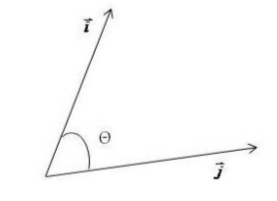
\includegraphics[height=0.35\columnwidth]{cosine}
\caption{The more the angle between the feature vectors, the lesser their similarity.}
\label{fig:cosine}
\end{figure}
\subsection{Cosine Similarity}
Items are represented as $m$ dimensional vectors (called feature vector), where each attribute represents a feature of the item. Items are characterized by the ordered set of values assigned to each feature. The similarity can then be viewed as the cosine of the angle between the two feature vectors as shown in Fig. \ref{fig:cosine}. Mathematically, it is defined as:
\begin{equation}
sim(\vec{a},\vec{b})=\cos\theta=\frac{\vec{a}\cdot\vec{b}}{\norm{\vec{a}}\cdot\norm{\vec{b}}}
\end{equation}

\subsection{Pearson Correlation Similarity}
Pearson Correlation Similarity measures correlation between two variables by computing the ratio of their co-variance and standard deviations. It is defined as:
\begin{equation}
p(x, y)=corr(x, y)=\frac{cov(x, y)}{\sigma_x\cdot\sigma_y} \nonumber
\end{equation}
In the domain of recommendation systems, it is used to find the correlation between items and users. Assume that both the items $a$ and $b$ have been rated by a set of users S. Let $R_{s,a}$ represent the rating given by user $s$ to item $a$. Further, let $\overline{R_a}$ denote the average rating for item $a$ over the complete user-space (who have rated $a$). The similarity measure is, then, defined as:
\begin{equation}
sim(a,b)=\frac{\sum_{s\in S} (R_{s,a}-\overline{R_a})(R_{s,b}-\overline{R_b})}{\sqrt{\sum_{s\in S} (R_{s,a}-\overline{R_a})^2}\sqrt{\sum_{s\in S} (R_{s,b}-\overline{R_b})^2}}
\end{equation}



